% !TEX root = Document.tex
\Chapter{Choix de capteurs}\label{sec:capteurs}
%\color{red}
%Intégrer ce chapitre à la revue de littérature? Ou faire un chapitre très court.
%\color{black}

Il va de soit que pour qu'un robot puisse éviter des obstacles et se déplacer de façon autonome, il doit avoir un moyen de percevoir son environnement. Dans ce chapitre nous traitons des capteurs utilisables dans le contexte de la navigation de robots mobiles et possiblement de la reconstruction 3D. En général, il existe trois sortes de capteurs utilisés: la vision passive, la vision active et diverses sortes de télémètres laser.

\section{Systèmes de vision passive}

Dans la section \ref{subsec:stereo_vision} nous avons touché le sujet de vision stéréo, un exemple de premier plan d'un capteur passif c'est-à-dire un capteur capable de percevoir un phénomène quelconque sans devoir émettre un signal. En effet, les caméras sont un moyen peu coûteux de percevoir la profondeur et sont couramment utilisés dans des micro-véhicules aériens commerciaux tel que le Yuneec Typhoon H dans la Figure \ref{fig:yuneec}. Par contre, la vision stéréo n'étant pas infaillible, la perception de profondeur peut échouer dans les environnement comportant peu de texture ou trop peu de lumière. Malgré certaines méthodes de régularisation pour tenter de remplir les trous en propageant l'information des régions aux alentours \citep{Hirschmuller2008}, l'état de l'art est à un point où les entreprises jugent encore prudent d'ajouter un capteur secondaire, tel qu'un sonar dans la Figure \ref{subfig:yuneec_closeup}, pour compenser les échecs de perception.

\begin{figure}[ht]
  \centering
  \subfloat[]{
  	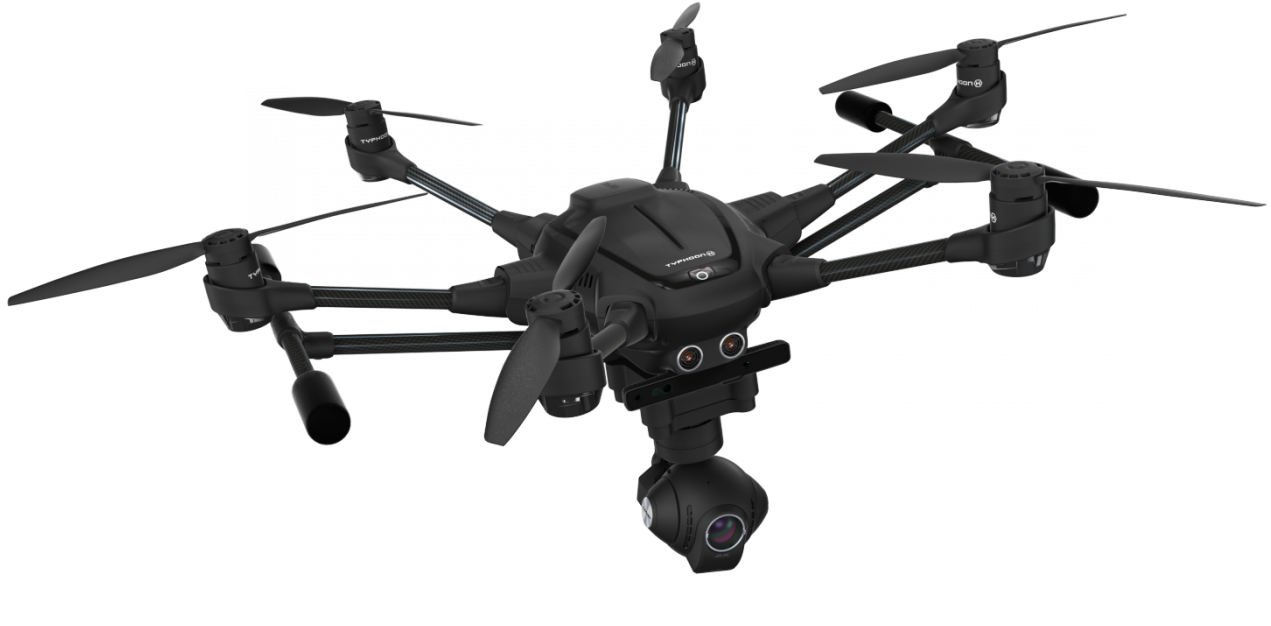
\includegraphics[width=0.60\linewidth]{images/yuneec_full.png}
  	\label{subfig:yuneec_full}
  }
  \hfil
  \subfloat[]{
  	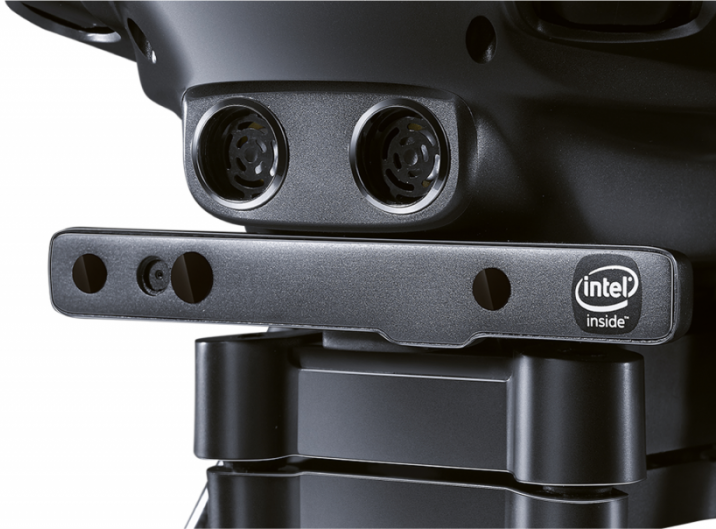
\includegraphics[width=0.35\linewidth]{images/yuneec_closeup.png}
  	\label{subfig:yuneec_closeup}
  }
  \caption[Systèmes de caméra stéréo augmentés de capteurs secondaires.]{
    (a) Le multi-rotor Yuneec Typhoon H (b) La caméra stéréo infrarouge Intel RealSense augmentée d'un sonar pour détecter les obstacles lors des échecs de perception.
  }
  \label{fig:yuneec}
\end{figure}

Dans le contexte des micro-véhicules aériens, il arrive parfois que l'on veuille miniaturiser et simplifier le système à un point où il serait désirable d'avoir un système monoculaire au lieu de stéréo. Tel que mentionné dans la section \ref{subsec:reconstruction} il est possible de mettre à l'échelle une carte 3D construite monoculairement au moyen d'une source d'information métrique secondaire tel qu'une centrale inertielle \citep{muratal2017vimonoslam}. Par contre, pour que cette carte soit utilisable pour la navigation, elle doit être construite de façon à pouvoir représenter les surfaces des obstacles. \cite{Yang2017} proposent de profiter de l'exactitude d'un système d'odométrie visuoinertiel pour construire des cartes de profondeur au moyen de résolution stéréo par mouvement. En d'autres mots, au lieu d'avoir deux caméras pour la triangulation de points, nous avons une seule caméra qui se déplace dans l'espace pour la triangulation.

\section{Systèmes de vision active}

Une autre façon de compenser pour les lacunes de la vision stéréo est d'utiliser la vision active, c'est-à-dire de projeter une onde quelconque pour en détecter le retour. L'un des exemples les mieux connus de ce type de système est la ligne de produits Microsoft Kinect. Originalement prévue pour permettre aux usager des consoles de jeux Xbox360 de jouer à des jeux contrôlés par gestuelle, la caméra de profondeur a rapidement été adoptée par le milieu académique pour son faible coût et sa précision relativement élevée \citep{khoshelham2012}. La Kinect pour Xbox360 fonctionnait originalement au moyen d'un projecteur laser quasi-infrarouge (NIR) et d'une caméra NIR. Suivant le principe de la \guillemotleft lumière structurée \guillemotright un motif NIR connu est projeté sur la scène et une caméra analysant la déformation du motif permet de calculer la profondeur de la scène \citep{Zhang2012}.

\begin{figure}[!h]
  \centering
  \subfloat[]{
    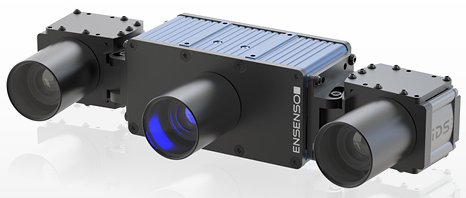
\includegraphics[width=0.5\linewidth]{images/ensenso3d.jpg}
    \label{subfig:ensenso}
  }
  \subfloat[]{
    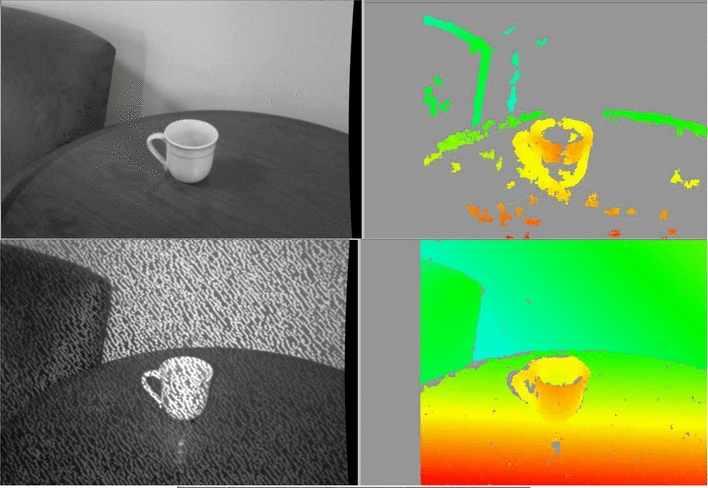
\includegraphics[width=0.4\linewidth]{images/konolidge_stereo.jpg}
    \label{subfig:kono_stereo}
  }
  \caption[Caméras 3D par projection de texture]{
    (a) Caméra Ensenso 3D fonctionnant par projection de texture et résolution stéréo.
    (b) Résultat de la méthode proposée par \citep{konolige2010}.
  }
  \label{fig:3d_cams}
\end{figure}

\cite{konolige2010} propose une méthode similaire où une caméra stéréo est augmentée d'un projecteur de texture pour permettre la résolution de la profondeur dans les scènes dépourvue de texture adéquate. La mise en correspondance des blocs stereo se fait avec la connaissance \textit{a priori} de la texture qui avait été projetée. À ce jour, ce principe est utilisé dans une variété de produits commerciaux tel que la caméra Ensenso 3D de IDS Imaging.

Par contre, les caméras par lumière structurée souffrent de plusieurs inconvénients, notamment leur sensibilité à la lumière infrarouge ambiante et leur imprécision dans le cas de scènes en mouvement \citep{khoshelham2012}. Dans les dernières cinq années, nous avons assisté à une baisse de prix considérables dans les capteurs de profondeur fonctionnant par \textit{time-of-flight (ToF)} (temps de vol). Le principe du ToF se résume à projeter périodiquement une lumière NIR modulée en intensité et d'en mesurer le temps de retour. Bien sûr, cette dernière n'est pas mesurée directement; elle est plutôt calculée à partir du déphasage du signal de retour capté par la caméra. L'avantage de caméras ToF est qu'elles offrent une bonne performance dans des environnements à haute et basse luminosité, en plus d'offrir un temps de réponse rapide. Encore ici, l'exemple le plus répandu d'une caméra ToF est la Microsoft Kinect v2 pour Xbox One.

Une dernière amélioration récente dans le domaine des caméras de profondeur est la ligne de produits Intel RealSense (ex. Figure \ref{subfig:yuneec_closeup}) fonctionnant par \textit{unstructured light} (lumière non-structurée) dont le traitement est accéléré par un circuit intégré à application dédiée (ASIC). Une texture fixe est projetée sur la scène au moyen d'un projecteur laser infrarouge. Cette texture est précalculée pour maximiser le contraste et pour miniser la similitude le long de l'axe de recherche épipolaire. À l'inverse de la Kinect 1, la texture est inconnue au moment de la résolution stéréo et ne sert qu'à   L'originalité de la solution provient du fait que la caméra stéréo infrarouge permet d'opérer une RealSense dans un environnement où la lumière du soleil est de forte intensité ainsi que dans la noirceur totale grâce au projecteur. De plus, la nature matérielle des caméras stéréo fait en sorte que la RealSense peut être produite à faible coût, dans un emballage petit et avec une consommation électrique relativement basse \citep{Keselman_2017_CVPR_Workshops}.

\section{Télémètres laser}

Un dernier type de capteur à considérer est le télémètre laser ou LIDAR pour \textit{Light Detection and Ranging}. Opérant souvent par ToF, les télémètres lasers sont combinés à des assemblages de moteurs et de miroirs pour obtenir des scanner laser en 2D ou 3D. L'un des exemples les plus médiatisés de l'utilisation de lidars pour la navigation de véhicules terrestres était Stanley, la voiture autonome de Stanford qui a gagné le DARPA Grand Challenge en 2005 \citep{thrun2006stanley}.

\begin{figure}[ht]
  \centering
  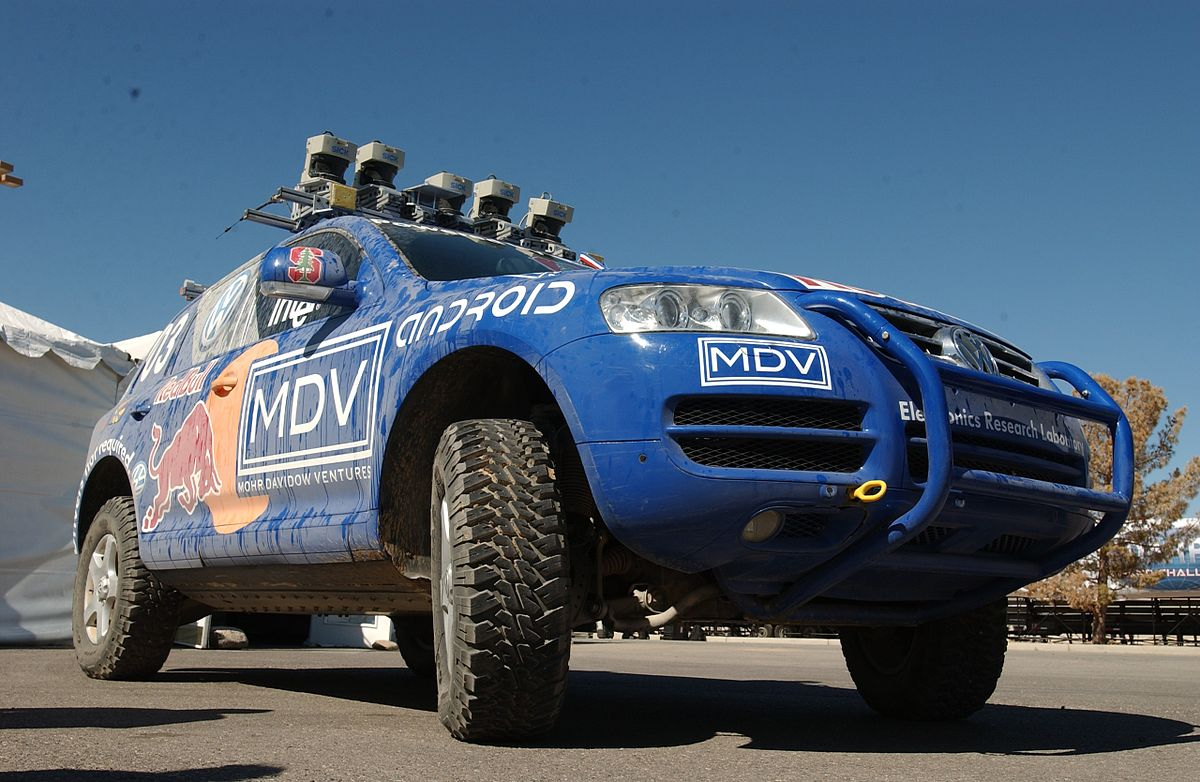
\includegraphics[width=0.5\linewidth]{images/stanley.jpg}
  \caption[Stanley la voiture autonome fonctionnant par lidar.]{Stanley était équipé de 5 lidar 2D sur son toit pour la détection d'obstacles et la navigation \citep{thrun2006stanley}.}
  \label{fig:stanley}
\end{figure}

Avec le temps, les lidars se sont améliorés pour devenir plus compacts et moins dispendieux à un point où il est possible de les installer sur des véhicules multi-rotors pour fins de cartographie et de localisation \citep{zhang2018aerial}. La tendance de miniaturisation se maintient avec l'arrivée récente sur le marché de lidars à état solide sans moteurs ou mirroirs pour la déflection du faisceau laser. Dans le chapitre \ref{sec:uav} nous démontrerons l'utilisation d'un tel capteur, le LeddarVu8 pour la navigation d'un véhicule aérien.

\begin{figure}[!h]
  \centering
  \subfloat[]{
    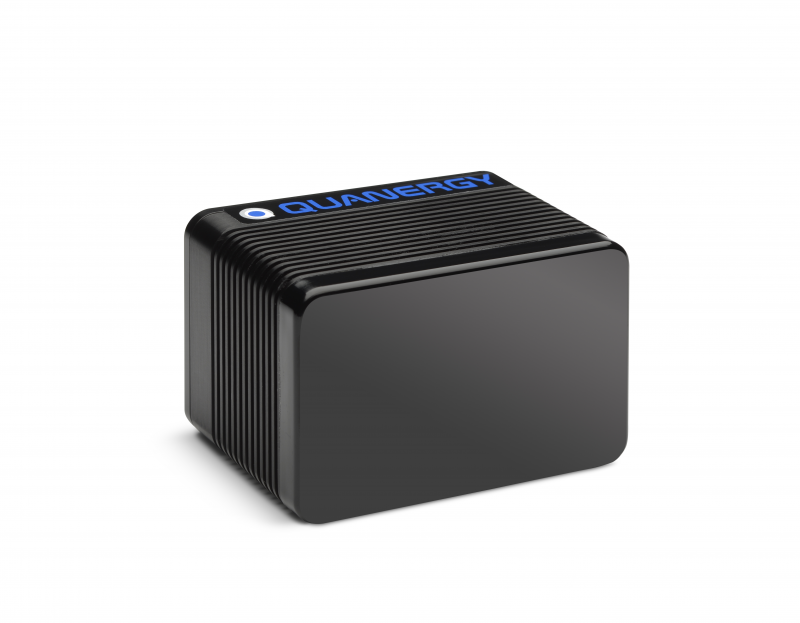
\includegraphics[width=0.5\linewidth]{images/quanergy.png}
    \label{subfig:quanergy}
  }
  \subfloat[]{
    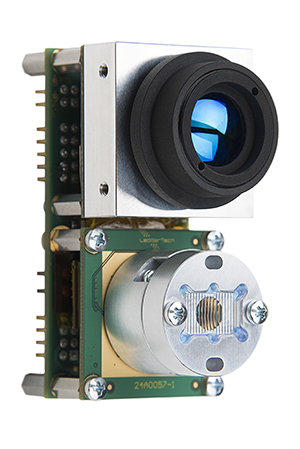
\includegraphics[width=0.2\linewidth]{images/leddar.jpg}
    \label{subfig:leddarvu}
  }
  \caption[Lidars à état solide]{
    (a) Le Quanergy S3 avec $8000$ points dans un angle de vue de $120^\circ$ horizontal et vertical \citep{eldada2016}.
    (b) Le LeddarVu8 avec $8$ segments de détection.
  }
  \label{fig:lidars}
\end{figure}
